\documentclass[article,a4paper,12pt,brazil,sumario=tradicional]{abntex2}
\usepackage{titlesec}

\setcounter{secnumdepth}{4}

\titleformat{\paragraph}
{\normalfont\normalsize}{\theparagraph}{1em}{}

\usepackage{array}
\usepackage{subfig}
\usepackage[utf8]{inputenc}
\usepackage{indentfirst}
\usepackage{hyperref}
\usepackage[hyphenbreaks]{breakurl}
\usepackage[alf,abnt-etal-text=it]{abntex2cite}
\usepackage[brazil]{babel}
\usepackage[space]{grffile}
\graphicspath{ {./images/} }
\setlength{\parindent}{3em}

\newcolumntype{C}[1]{>{\centering\arraybackslash\hspace{0pt}}p{#1}}

\setlrmarginsandblock{3cm}{3cm}{*}
\setulmarginsandblock{3cm}{2cm}{*}
\checkandfixthelayout

\titleformat{\section}{\normalfont\normalsize\bfseries}{\thesection.}{1em}{\MakeUppercase}
\titleformat{\subsection}{\normalfont\normalsize}{\thesubsection.}{1em}{\MakeUppercase}
\titleformat{\subsubsection}{\normalfont\normalsize\bfseries}{\thesubsubsection.}{1em}{}

\renewenvironment{quotation}
  {\small\list{}{\rightmargin=0cm \leftmargin=2cm}%
   \item\relax}
  {\endlist}
  
\hypersetup{%
    pdfborder = {0 0 0}
}

\title{ {\Large Título\footnote{Trabalho de conclusão de curso apresentado ao curso de Bacharelado em Sistemas de Informação da Universidade Federal Fluminense como requisito parcial para conclusão do curso.}\\\\
\vspace{.2} 
\textit{Titulo}\\}}

\date{ }

\begin{document}

\textual

\begin{center}
{\Large Título em português\footnote{Trabalho de conclusão de curso apresentado ao curso de Bacharelado em Sistemas de Informação da Universidade Federal Fluminense como requisito parcial para conclusão do curso.}

\textit{Comparativo de custo de tratamento para epilepsia no estado do Rio de Janeiro}\\}
\end{center}
\vspace{.2cm} 

\begin{flushright}
Bruno Moraes Cotelo\footnote{Graduando do Curso de Sistemas de Informação - UFF, bruno\_cotelo@id.uff.br}

Tiago Rodrigues de Matos\footnote{Graduando do Curso de Sistemas de Informação - UFF, ti\_matos@id.uff.br}

Daniel Cardoso Moraes de Oliveira\footnote{Orientador - Instituto de Computação - UFF, danielcmo@ic.uff.br.} 

Nome completo do coorientador\footnote{Coorientador - vínculo institucional do coorientador, e-mail do coorientador.}
\end{flushright}

\vspace{\onelineskip}

\begin{center}
    \textbf{Resumo}
\end{center}

\vspace{-.3cm}

\noindent Este estudo aprofundado investiga os custos do tratamento da epilepsia no Rio de Janeiro entre 2015 e 2023, focando no sistema público de saúde (SIASUS). O objetivo principal é comparar os custos do tratamento convencional com medicamentos antiepilépticos (MAEs) e o tratamento com canabidiol (CBD) em diferentes graus da doença..

\vspace{.4cm}
 
\noindent
\textbf{Palavras-chaves}: Epilepsia, Tratamento convencional, Canabidiol, Custos diretos, Custos indiretos, Graus da doença, Transições de estado, SIASUS, Rio de Janeiro.. 
 
\vspace{\onelineskip}

\begin{center}
    \textbf{Abstract}
\end{center}

\vspace{-.3cm}
\begin{hyphenrules}{english}
\noindent This comprehensive study delves into the intricate costs of epilepsy treatment in Rio de Janeiro between 2015 and 2023, with a specific focus on the public health system (SIASUS). The primary objective is to conduct a meticulous comparison of the financial implications associated with conventional treatment using antiepileptic drugs (AEDs) and the emerging alternative of cannabidiol (CBD) therapy, taking into account the varying degrees of epilepsy severity.
\end{hyphenrules}
\vspace{.4cm}
 
\noindent \textbf{Keywords}: Epilepsy, Conventional treatment, Cannabidiol, Direct costs, Indirect costs, Degrees of Disease, State transitions, SIASUS, Rio de Janeiro.

\vspace{.4cm}

\noindent \textbf{Aprovado em:} dd/mm/aaaa.~~~\textbf{Versão Final em:} dd/mm/aaaa

\section{Introdução}

O termo epilepsia se refere a um distúrbio da atividade cerebral caracterizada pela ocorrência periódica e espontânea de atividade elétrica altamente sincronizada, acompanhada de manifestações comportamentais. Dessa forma, não é uma unica doenca ou sindrome, e sim um grupo de disturbios que ocorrem a partir de funcoes cerebrais alteradas. (Fonte: Alterações cardiovasculares e morte súbita nas epilepsias)  

Esse disturbio pode ocorrer motivado por diversos fatores, como febre, intoxicacao, alteracoes vasculares ou doencas degenerativas. Atualmente, a epilepsia acomete cerca de 2\% da populacão brasileira, e cerca de 50 milhões de pessoas no mundo (Fonte GOV.BR(Na resolucao da CONITEC diz 65M)). No Brasil é possivel receber atendimento integral e gratuito a partir do Sistema Unico de Saude (SUS), tendo 29 estabelecimentos habilitados para tratamento de alta complexidade em neurologia/neurocirurgia para abranger desde consultas, exames, diagnosticos, tratamento e fornecimento de medicamentos.

O uso medicamentos para ajudar a controlar as crises faz com que os pacientes que sofrem dessa doenca possam viver sem grandes limitacoes. Porem, cerca de 30\% desses pacientes ainda apresentam casos de crises, sendo considerados refratários ao tratamento. No SUS, segundo o Protocolo Clinico e Diretrizes Terapeuticas (PCDT) para epilepsia, publicado em 2018, são disponibilizados cerca de 13 medicamentos distintos para o tratamento, que deve ser iniciado com a prescricao de apenas um, podendo, em caso de falha, ser alterado ou feita a combinacao de dois desses medicamentos antiepilépticos. Em caso de persistencia nas crises com o tratamento medicamentoso, o SUS oferece como opcao a realizacao de uma cirurgia ou procedimento de estimulacao elétrica do nervo vago (Fonte: Resolucao CONITEC).

\section{Desenvolvimento}

Parte principal do artigo, que contém a exposição ordenada e pormenorizada do assunto tratado. 

\subsection{Citações}

As citações apresentadas no artigo seguirão as normas de apresentação de acordo com a NBR 10520:2002 ~\cite{bibliografica6023}. Para chamada das citações será adotado o sistema ``autor-dat'' em todo artigo. As chamadas incluídas na sentença devem ser em letras maiúsculas e minúsculas e, quando estiverem entre parênteses devem ser em letras maiúsculas. Nas citações diretas devem ser especificadas a(s) página(a) da fonte consultada; para citações indiretas este item é opcional. Todas as obras citadas deverão aparecer na lista de referências, e não, em notas de rodapé.

De acordo com Associação Brasileira de Normas Técnicas (~\citeyear{bibliografica6023}), ``as citações diretas, no texto, com até três linhas, devem estar contidas entre aspas duplas''.

\begin{quotation}
\noindent
As citações diretas, no texto, com mais de três linhas, devem ser destacadas com recuo de 4cm da margem esquerda, com letra menor que a do texto e sem aspas ~\cite{bibliografica6023}.
\end{quotation}

\subsection{Notas de rodapé}

As notas de rodapé devem ser utilizadas apenas para notas explicativas, ou seja, usadas para comentários, esclarecimentos ou explanações que não possam ser incluídos no texto. A numeração das notas é feita em algarismos arábicos, de forma única e consecutiva.

\subsection{Numeração progressiva}

A numeração progressiva das seções no desenvolvimento do artigo deve atender às especificações da ABNT NBR 6024:2012. As seções devem se limitar até a seção quinária e seus títulos devem ser destacados tipograficamente, de forma hierárquica, através de recursos gráficos de maiúscula, negrito, itálico ou sublinhado e outros.

\subsection{Figuras e tabelas}

Todas as figuras e tabelas devem ser numeradas em ordem crescente, na sequencia que são citadas no corpo do artigo. As figuras e tabelas devem ser exibidas preferencialmente logo após o parágrafo onde ela é citada. Todas as figuras e tabelas devem ser citadas no corpo do texto. O posicionamento da legenda é logo abaixo da figura, conforme exemplificado na Figura~\ref{fig:exampleFig1}.

\begin{figure}[!ht]
\centering
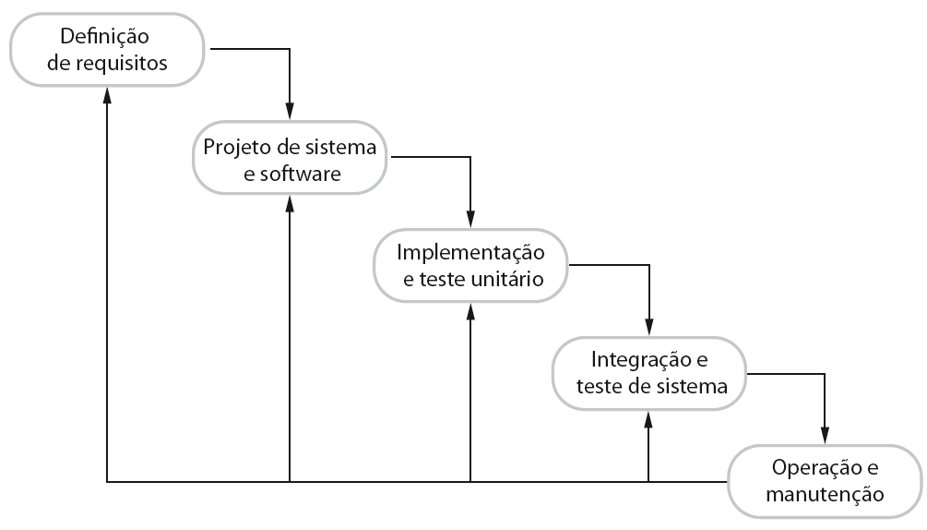
\includegraphics[width=1\textwidth]{Imagem1.png}
\caption{Modelo do processo de desenvolvimento de software em cascata. Fonte: \cite{sommerville2011software}.}
\label{fig:exampleFig1}
\end{figure}

Nas tabelas, tente evitar o uso de fundos coloridos ou sombreados e evite linhas de enquadramento grossas, dobradas ou desnecessárias. Ao relatar dados empíricos, não use mais dígitos decimais do que o garantido por sua precisão e reprodutibilidade. A legenda da tabela deve ser colocada acima da tabela (consulte a Tabela~\ref{tab:exTable1}).

\begin{table}[!ht]
\centering
\caption{Taxa de sucesso de projetos de desenvolvimento de software pelo tamanho do projeto. Fonte: \cite{clancy1995standish}.}
      \begin{tabular}{| p{3cm} | C{2cm} | C{2cm} | C{2cm} |}
        \hline
        & Bem sucedido & Deficitário & Falho \\ \hline
        Muito grande & 2 & 7 & 17 \\ \hline
        Grande & 6 & 17 & 24 \\ \hline
        Médio & 9 & 26 & 31 \\ \hline
        Pequeno & 21 & 32 & 17 \\ \hline
        Muito pequeno & 62 & 16 & 11 \\ \hline
        \textbf{TOTAL} & \textbf{100} & \textbf{100} & \textbf{100} \\ \hline
    \end{tabular}
    \label{tab:exTable1}
\end{table}

\subsection{Referências}

As referências bibliográficas devem ficar localizadas ao final do texto, contendo exclusivamente as obras citadas, ordenadas em uma única ordem alfabética e de acordo com as normas vigentes da ABNT NBR 6023/2018. Devem ser digitadas com espaçamento simples entre linhas e separadas entre si por um espaço simples em branco. O alinhamento do texto deve ser à esquerda.

A expressão ``Referências'' deve figurar de forma centralizada e não numerada, com o mesmo destaque tipográfico das seções primárias e logo após a conclusão.

Para esclarecimentos, consultar a norma correspondente.

\section{Conclusão}

Parte final do artigo, na qual se apresentam as considerações correspondentes aos objetivos e/ou hipóteses.

\newpage
\bibliography{references}

\newpage
\renewcommand{\listfigurename}{APÊNDICE A - Lista de ilustrações}
\listoffigures

\newpage
\renewcommand{\listtablename}{APÊNDICE B - Lista de tabelas}
\listoftables

\begin{appendices}
\newpage
\chapter* {APÊNDICE C}
\noindent
Os apêndices A e B devem conter a lista de ilustrações e tabelas, respectivamente. Os apêndices seguintes podem ser usados para apresentar textos elaborados pelo próprio autor, a fim de complementar a sua argumentação. Por exemplo, no caso de desenvolvimento de sistemas, podem constar nos apêndices os artefatos gerados da análise de sistemas, como protótipos de telas, casos de uso, diagramas UML, ou a lista de requisitos de negócio e de usuário.

\newpage
\chapter*{ANEXO A}
\noindent
Seção opcional. Anexos são os documentos de autoria externa, ou não elaborados pelo autor, que servem de fundamentação, comprovação ou ilustração.
\end{appendices}

\newpage
\chapter*{Agradecimentos}
\noindent
Seção opcional. Oportunidade para o(s) autor(es) registrar(em) os agradecimentos, em especial, quando o artigo recebeu ajuda financeira de alguma instituição de fomento, ou represente o resultado de um trabalho colaborativo ou multidisciplinar, envolvendo áreas externas ao Instituto de Computação.

\end{document}
